\documentclass[12pt,twoside]{article}
\usepackage[dvipsnames]{xcolor}
\usepackage{tikz,graphicx,amsmath,amsfonts,amscd,amssymb,bm,cite,epsfig,epsf,url}
\usepackage[hang,flushmargin]{footmisc}
\usepackage[colorlinks=true,urlcolor=blue,citecolor=blue]{hyperref}
\usepackage{amsthm,multirow,wasysym,appendix}
\usepackage{array,subcaption} 
% \usepackage[small,bf]{caption}
\usepackage{bbm}
\usepackage{pgfplots}
\usetikzlibrary{spy}
\usepgfplotslibrary{external}
\usepgfplotslibrary{fillbetween}
\usetikzlibrary{arrows,automata}
\usepackage{thmtools}
\usepackage{blkarray} 
\usepackage{textcomp}
\usepackage[left=0.8in,right=1.0in,top=1.0in,bottom=1.0in]{geometry}

\usepackage{times}
\usepackage{amsfonts}
\usepackage{amsmath}
%\usepackage[psamsfonts]{amssymb}
\usepackage{latexsym}
\usepackage{color}
\usepackage{graphics}
\usepackage{enumerate}
\usepackage{amstext}
\usepackage{blkarray}
\usepackage{url}
\usepackage{epsfig}
\usepackage{bm}
\usepackage{hyperref}
\hypersetup{
    colorlinks=true,
    linkcolor=blue,
    filecolor=magenta,      
    urlcolor=blue,
}
\usepackage{mathtools}
\usepackage{minted}

%% Probability operators and functions
%
% \def \P{\mathrm{P}}
\def \P{\mathrm{P}}
\def \E{\mathrm{E}}
\def \Var{\mathrm{Var}}
\let\var\Var
\def \Cov {\mathrm{Cov}} \let\cov\Cov
\def \MSE {\mathrm{MSE}} \let\mse\MSE
\def \sgn {\mathrm{sgn}}
\def \R {\mathbb{R}}
\def \C {\mathbb{C}}
\def \N {\mathbb{N}}
\def \Z {\mathbb{Z}}
\def \cV {\mathcal{V}}
\def \cS {\mathcal{S}}
\DeclareMathOperator*{\argmin}{arg\,min}
\DeclareMathOperator*{\argmax}{arg\,max}
\newcommand{\red}[1]{\textcolor{red}{#1}}
\newcommand{\blue}[1]{\textcolor{blue}{#1}}
\newcommand{\green}[1]{\textcolor{ForestGreen}{ #1}}
\newcommand{\fuchsia}[1]{\textcolor{RoyalPurple}{ #1}}

%
%% Probability distributions
%
%\def \Bern    {\mathrm{Bern}}
%\def \Binom   {\mathrm{Binom}}
%\def \Exp     {\mathrm{Exp}}
%\def \Geom    {\mathrm{Geom}}
%\def \Norm    {\mathcal{N}}
%\def \Poisson {\mathrm{Poisson}}
%\def \Unif    {\mathrm {U}}
%
\newcommand{\bdb}[1]{\textcolor{red}{#1}}

\newcommand{\ml}[1]{\mathcal{ #1 } }
\newcommand{\wh}[1]{\widehat{ #1 } }
\newcommand{\wt}[1]{\widetilde{ #1 } }
\newcommand{\conj}[1]{\overline{ #1 } }
\newcommand{\rnd}[1]{\tilde{ #1 } }
\newcommand{\rv}[1]{ \rnd{ #1}  }
\newcommand{\rx}{\rnd{ x}  }
\newcommand{\ry}{\rnd{ y}  }
\newcommand{\ra}{\rnd{ a}  }
\newcommand{\rb}{\rnd{ b}  }
\newcommand{\rpc}{\widetilde{ pc}  }

\def \cnd {\, | \,}
\def \Id { I }
\def \J {\mathbf{1}\mathbf{1}^T}

\newcommand{\op}[1]{\operatorname{#1}}
\newcommand{\setdef}[2]{ := \keys{ #1 \; | \; #2 } }
\newcommand{\set}[2]{ \keys{ #1 \; | \; #2 } }
\newcommand{\sign}[1]{\op{sign}\left( #1 \right) }
\newcommand{\trace}[1]{\op{tr}\left( #1 \right) }
\newcommand{\tr}[1]{\op{tr}\left( #1 \right) }
\newcommand{\inv}[1]{\left( #1 \right)^{-1} }
\newcommand{\abs}[1]{\left| #1 \right|}
\newcommand{\sabs}[1]{| #1 |}
\newcommand{\keys}[1]{\left\{ #1 \right\}}
\newcommand{\sqbr}[1]{\left[ #1 \right]}
\newcommand{\sbrac}[1]{ ( #1 ) }
\newcommand{\brac}[1]{\left( #1 \right) }
\newcommand{\bbrac}[1]{\big( #1 \big) }
\newcommand{\Bbrac}[1]{\Big( #1 \Big)}
\newcommand{\BBbrac}[1]{\BIG( #1 \Big)}
\newcommand{\MAT}[1]{\begin{bmatrix} #1 \end{bmatrix}}
\newcommand{\sMAT}[1]{\left(\begin{smallmatrix} #1 \end{smallmatrix}\right)}
\newcommand{\sMATn}[1]{\begin{smallmatrix} #1 \end{smallmatrix}}
\newcommand{\PROD}[2]{\left \langle #1, #2\right \rangle}
\newcommand{\PRODs}[2]{\langle #1, #2 \rangle}
\newcommand{\der}[2]{\frac{\text{d}#2}{\text{d}#1}}
\newcommand{\pder}[2]{\frac{\partial#2}{\partial#1}}
\newcommand{\derTwo}[2]{\frac{\text{d}^2#2}{\text{d}#1^2}}
\newcommand{\ceil}[1]{\lceil #1 \rceil}
\newcommand{\Imag}[1]{\op{Im}\brac{ #1 }}
\newcommand{\Real}[1]{\op{Re}\brac{ #1 }}
\newcommand{\norm}[1]{\left|\left| #1 \right|\right| }
\newcommand{\norms}[1]{ \| #1 \|  }
\newcommand{\normProd}[1]{\left|\left| #1 \right|\right| _{\PROD{\cdot}{\cdot}} }
\newcommand{\normTwo}[1]{\left|\left| #1 \right|\right| _{2} }
\newcommand{\normTwos}[1]{ \| #1  \| _{2} }
\newcommand{\normZero}[1]{\left|\left| #1 \right|\right| _{0} }
\newcommand{\normTV}[1]{\left|\left| #1 \right|\right|  _{ \op{TV}  } }% _{\op{c} \ell_1} }
\newcommand{\normOne}[1]{\left|\left| #1 \right|\right| _{1} }
\newcommand{\normOnes}[1]{\| #1 \| _{1} }
\newcommand{\normOneTwo}[1]{\left|\left| #1 \right|\right| _{1,2} }
\newcommand{\normF}[1]{\left|\left| #1 \right|\right| _{\op{F}} }
\newcommand{\normLTwo}[1]{\left|\left| #1 \right|\right| _{\ml{L}_2} }
\newcommand{\normNuc}[1]{\left|\left| #1 \right|\right| _{\ast} }
\newcommand{\normOp}[1]{\left|\left| #1 \right|\right|  }
\newcommand{\normInf}[1]{\left|\left| #1 \right|\right| _{\infty}  }
\newcommand{\proj}[1]{\mathcal{P}_{#1} \, }
\newcommand{\diff}[1]{ \, \text{d}#1 }
\newcommand{\vc}[1]{\boldsymbol{\vec{#1}}}
\newcommand{\rc}[1]{\boldsymbol{#1}}
\newcommand{\vx}{\vec{x}}
\newcommand{\vy}{\vec{y}}
\newcommand{\vz}{\vec{z}}
\newcommand{\vu}{\vec{u}}
\newcommand{\vv}{\vec{v}}
\newcommand{\vb}{\vec{\beta}}
\newcommand{\va}{\vec{\alpha}}
\newcommand{\vaa}{\vec{a}}
\newcommand{\vbb}{\vec{b}}
\newcommand{\vg}{\vec{g}}
\newcommand{\vw}{\vec{w}}
\newcommand{\vh}{\vec{h}}
\newcommand{\vnu}{\vec{\nu}}
\newcommand{\rvnu}{\vc{\nu}}

\newtheorem{theorem}{Theorem}[section]
% \declaretheorem[style=plain,qed=$\square$]{theorem}
\newtheorem{corollary}[theorem]{Corollary}
\newtheorem{definition}[theorem]{Definition}
\newtheorem{lemma}[theorem]{Lemma}
\newtheorem{remark}[theorem]{Remark}
\newtheorem{algorithm}[theorem]{Algorithm}

% \theoremstyle{definition}
%\newtheorem{example}[proof]{Example}
%\declaretheorem[style=definition,qed=$\triangle$,sibling=definition]{example}
%\declaretheorem[style=definition,qed=$\bigcirc$,sibling=definition]{application}

%
%% Typographic tweaks and miscellaneous
%\newcommand{\sfrac}[2]{\mbox{\small$\displaystyle\frac{#1}{#2}$}}
%\newcommand{\suchthat}{\kern0.1em{:}\kern0.3em}
%\newcommand{\qqquad}{\kern3em}
%\newcommand{\cond}{\,|\,}
%\def\Matlab{\textsc{Matlab}}
%\newcommand{\displayskip}[1]{\abovedisplayskip #1\belowdisplayskip #1}
%\newcommand{\term}[1]{\emph{#1}}
%\renewcommand{\implies}{\;\Rightarrow\;}

% My macros

\def\Kset{\mathbb{K}}
\def\Nset{\mathbb{N}}
\def\Qset{\mathbb{Q}}
\def\Rset{\mathbb{R}}
\def\Sset{\mathbb{S}}
\def\Zset{\mathbb{Z}}
\def\squareforqed{\hbox{\rlap{$\sqcap$}$\sqcup$}}
\def\qed{\ifmmode\squareforqed\else{\unskip\nobreak\hfil
\penalty50\hskip1em\null\nobreak\hfil\squareforqed
\parfillskip=0pt\finalhyphendemerits=0\endgraf}\fi}

%\DeclareMathOperator*{\E}{\rm E}
%\DeclareMathOperator*{\argmax}{\rm argmax}
%\DeclareMathOperator*{\argmin}{\rm argmin}
%\DeclareMathOperator{\sgn}{sign}
\DeclareMathOperator{\supp}{supp}
\DeclareMathOperator{\last}{last}
%\DeclareMathOperator{\sign}{\sgn}
\DeclareMathOperator{\diag}{diag}
\providecommand{\abs}[1]{\lvert#1\rvert}
\providecommand{\norm}[1]{\lVert#1\rVert}
\def\vcdim{\textnormal{VCdim}}
\DeclareMathOperator*{\B}{\textbf{B}}

%\DeclarePairedDelimiter\ceil{\lceil}{\rceil}
%\DeclarePairedDelimiter\floor{\lfloor}{\rfloor}

\newcommand{\cX}{{\mathcal X}}
\newcommand{\cY}{{\mathcal Y}}
\newcommand{\cA}{{\mathcal A}}
\newcommand{\ignore}[1]{}
\newcommand{\bi}{\begin{itemize}}
\newcommand{\ei}{\end{itemize}}
\newcommand{\be}{\begin{enumerate}}
\newcommand{\ee}{\end{enumerate}}
\newcommand{\bd}{\begin{description}}
\newcommand{\ed}{\end{description}}
\newcommand{\h}{\widehat}
\newcommand{\e}{\epsilon}
\newcommand{\mat}[1]{{\mathbf #1}}
%\newcommand{\R}{\mat{R}}
\newcommand{\0}{\mat{0}}
\newcommand{\M}{\mat{M}}

\newcommand{\D}{\mat{D}}
\renewcommand{\r}{\mat{r}}
\newcommand{\x}{\mat{x}}
\renewcommand{\u}{\mat{u}}
\renewcommand{\v}{\mat{v}}
\newcommand{\w}{\mat{w}}
\renewcommand{\H}{\text{0}}
\newcommand{\T}{\text{1}}
%\newcommand{\set}[1]{\{#1\}}
\newcommand{\xxi}{{\boldsymbol \xi}}
\newcommand{\ssigma}{{\boldsymbol \sigma}}
\newcommand{\Alpha}{{\boldsymbol \alpha}}
\newcommand{\tts}{\tt \small}
\newcommand{\hint}{\emph{hint}}
\newcommand{\matr}[1]{\bm{#1}}     % ISO complying version
\newcommand{\vect}[1]{\bm{#1}} % vectors

%\newcommand{\Var}{\mathrm{Var}}
%\newcommand{\Cov}{\mathrm{Cov}}

% New commands
\newcommand{\SP}{\mathbf{S}_{+}^n}
\newcommand{\Proj}{\mathcal{P}_{\mathcal{S}}}
\DeclarePairedDelimiterX{\inp}[2]{\langle}{\rangle}{#1, #2}
\newtheorem{proof}{Proof}


\begin{document}

\noindent DS-GA.1013 Mathematical Tools for Data Science \\
Homework 1 \\
Yves Greatti - yg390\\


\begin{enumerate}
\item (Rotation) For a symmetric matrix $A$, can there be a nonzero vector $x$ such that $Ax$ is nonzero and orthogonal to $x$? Either prove that this is impossible, or explain under what condition on the eigenvalues of $A$ such a vector exists.
Let $x \in V, x \neq 0$, an inner product space , by the spectral theorem there exists an orthonormal basis of  $V$, consisting of eigenvectors of $A$, let $u_1$, \ldots, $u_n$ be the eigenbasis of $A$, and $\lambda_1, \ldots, \lambda_n$ the eigenvalues for each of these eigenvectors.
$x \in \text{span}\{u_1, \ldots, u_n \} \Rightarrow  x=\sum_{i=1,n} \alpha_i u_i, \alpha_i \neq 0$.  $x^T (Ax) = (\sum_{i=1,n} \alpha_i u_i) (\sum_{j=1,n} \alpha_j A u_j) =  (\sum_{i=1,n} \alpha_i u_i) (\sum_{j=1,n} \alpha_j \lambda_j u_j) = \sum_{i=1,n} \alpha_i^2 \lambda_i$ since $u_i^T u_j = 0$ for $i \neq j$ and $u_i^T u_i =1$. $Ax$ is orthogonal to $x$: $x^T (Ax) = 0 \Rightarrow  \sum_{i=1,n} \alpha_i^2 \lambda_i = 0$.

\item (Matrix decomposition) The trace can be used to define an inner product between matrices:
\begin{align}
\PROD{A}{B} := \trace{A^TB}, \quad A,B \in \R^{m \times n},
\end{align}
where the corresponding norm is the Frobenius norm $\normF{A}:=\PROD{A}{A}$.
\begin{enumerate}
\item Express the inner product in terms of vectorized matrices and use the result to prove that this is a valid inner product.
$(A B)_{ij} = (\sum_k A_{ik} B_{kj})_{ij}$, and $(A^TB) _{ij} = (\sum_k A_{ki} B_{kj})_{ij}$.
$\trace{A} = \sum_i A_{ii}  \Rightarrow \trace{A^TB} = \sum_i \sum_k A_{ki} B_{ki} = \sum_i \sum_j A_{ij} B_{ij} = \text{vec}(A)^T \text{vect}(B) = \PROD{\text{vec}(A)} {\text{vec}(B)}$.
The trace is then the inner product between vectors in $\R^{mn}$ thus is a valid inner product.

\item Prove that for any $A,B \in \R^{m \times n}$, $\trace{A^TB}=\trace{BA^T}$.
$\trace{BA^T} =  \sum_i \sum_k B_{ik} A_{ik} =  \sum_i \sum_j A_{ij} B_{ij} =  \trace{A^TB}$.

\item Let $u_1$, \ldots, $u_n$ be the eigenvectors of a symmetric matrix $A$. Compute the inner product between the rank-1 matrices $u_iu_i^T$ and $u_ju_j^T$ for $i \neq j$, and also the norm of $u_iu_i^T$ for $i=1,\ldots,n$. 
For $i \neq j$, $\PROD{u_iu_i^T}{u_ju_j^T} = \trace{u_iu_i^Tu_ju_j^T} = \trace{u_i \; 0 \; u_j^T} = 0$, since $u_i, u_j$ are two eigenvectors of a symmetric matrix therefore orthogonal.
if $i=j$ then  $\PROD{u_iu_i^T}{u_iu_i^T} = \trace{u_iu_i^Tu_iu_i^T} =  \trace{u_i^T \; I \; u_i} = \trace{u_i^Tu_i} = 1$ if the eigenvectors are also orthonormal.
\item What is the projection of $A$ onto $u_iu_i^T$?
If $A$ is a symmetric matrix, by the spectral theorem, $A=U D U^T$ where $D$ is the diagonal matrix having $\lambda_i, i=1, \ldots,n$ the eigenvalues of $A$ on the diagonal.  Then $A = \sum_i \lambda_i u_i u_i^T$,  where $u_1$, \ldots, $u_n$ are the eigenvectors of A. The projection of $A$ onto $u_iu_i^T$ is $\PROD{A}{u_iu_i^T}$ thus
\begin{align*}
	\PROD{A}{u_iu_i^T}	&= 	\PROD{\sum_{j=1}^n  \lambda_j u_j u_j^T} {u_i u_i^T} \\
					&=	\sum_{j=1}^n\PROD{\lambda_j u_j u_j^T} {u_i u_i^T} \\
					&= 	\sum_{j=1}^n \lambda_j \PROD{u_j u_j^T} {u_i u_i^T} \\
					&=	 \lambda_i \PROD{u_i u_i^T} {u_i u_i^T} \\
					&= 	 \lambda_i 
\end{align*}
Where we applied linearity of the inner product for equations 2 and 3 and reuse the results of the inner product between eigenvectors from the previous question (assuming we chose eigenvectors orthonormal).

\item Provide a geometric interpretation of the matrix $A':=A-\lambda_1 u_1u_1^T$, which we defined in the proof of the spectral theorem, based on your previous answers.
From the previous question the orthogonal projection of A in $u_iu_i^T$ is $\lambda_i u_iu_i^T$ so $A' = \sum_i \lambda_i u_iu_i^T, i \neq 1$ has row or column subspaces contained in  $(u_1)^\bot$.

\end{enumerate}

\item (Quadratic forms) Let $A\in \R^{n \times n}$ be a symmetric matrix, and let $f(x):=x^TAx$ be the corresponding quadratic form. We consider the 1D function $g_{v}(t)=f(tv)$ obtained by restricting the quadratic form to lie in the direction of a vector $v$ with unit $\ell_2$ norm.
\begin{enumerate}
\item Is $g_{v}(t)$ a polynomial? If so, what kind?
	$g_{v}(t) = f(tv) = (tv)^T A (tv) = t^2 v^T A v = v^T A v \; t^2$, $v^T A v$ is a scalar, and $g_{v}(t)$ is a second-order polynomial in $t$. 
\item What is the curvature (i.e. the second derivative) of $g_{v}(t)=f(tv)$ at an arbitrary point $t$?
$g'_{v}(t)= 2 v^T A v \; t$ and the curvature is $g''_{v}(t)= 2 v^T A v$

\item What are the directions of maximum and minimum curvature of the quadratic form? What are the corresponding curvatures equal to?
By the spectral theorem, $A = U \textbf{diag}(\lambda) U^T$ where $\textbf{diag}$ is the diagonal matrix with on the diagonal: $\lambda_1 \ge \lambda_2 \ge \ldots \lambda_n$, which are the eigenvalues and $u_1, \dots, u_n$ the corresponding eigenvectors. The largest eigenvalue is
$\lambda_1 = \max_{\|v\|_2 =1} v^T A v$ with eigenvector $u_1 = \arg \max_{\|v\|_2 =1} v^T A v$, and the smaller eigenvalue  is given by $\lambda_n = \max_{\|v\|_2 =1} v^T A v, u_n = \arg \max_{\|v\|_2 =1} v^T A v$. Thus the maximum curvature is given by the largest eigenvalue $\lambda_1$ and  is in the direction of the corresponding eigenvector $u_1$. 
	The smallest curvature is  given  by  the  smallest  eigenvalue $\lambda_n$ and is in the direction of the corresponding eigenvector $u_n$.

\end{enumerate}

\item (Projected gradient ascent) Projected gradient descent is a method designed to find the maximum of a differentiable function $f:\R^n \rightarrow \R$ in a constraint set $\ml{S}$. Let $\ml{P}_{\ml{S}}$ denote the projection onto $\ml{S}$, i.e.
\begin{align}
\ml{P}_{\ml{S}}(x) := \arg \min_{y \in \ml{S}} \normTwo{x-y}^2.
\end{align} 
The $k$th update of projected gradient ascent equals
\begin{align}
x^{[k]} :=\ml{P}_{\ml{S}}( x^{[k-1]} + \alpha \nabla f (x^{[k-1]}) ), \qquad k=1,2,\ldots,
\end{align}
where $\alpha$ is a positive constant and $x^{[0]}$ is an arbitrary initial point.
\begin{enumerate}
\item Use the same arguments we used to prove Lemmas 5.1 and 5.2 in the notes on PCA to derive the projection of a vector $x$ onto the unit sphere in $n$ dimensions.
Let define $f(x) =  \normTwo{x-y}^2,y \in \ml{S}$, the directional derivative cannot be different than zero $f'_v(x) = \PROD{\nabla{x}}{v} = 0$ for any $v$ such that $x+ \epsilon v$ is on the sphere $\ml{S}$. Let $g(x)=x^T x, \| y \|_2 = 1$, $g$ describes points on the surface of the unit sphere. $x +\epsilon v$ is in the tangent  plane of $g$ at $x$ if $\nabla{g(x)}^T v = 0$, and for $\epsilon \approx 0$, $g(x + \epsilon v) \approx g(x)$. We are then looking for global minimizer points (global because $f$ is convex), where the level curves of $f$ are tangent to the curve $g$, or where the gradients are colinear. $\nabla_x{f(x)} = \nabla_x{(x^T x -2 x^T y + y^T y)} = 2 (x-y)$ and $\nabla_x{g(x)} = 2 x$, thus the projection of $x$ on $\ml{S}$, $y_p$, verifies $x -y_p = \lambda x$ or $y_p = (1- \lambda) x$. for any vector $y \in \ml{S}$, we have $y = (1-\lambda) x + x_\bot$ where $x_\bot$ is in the hyperplane orthogonal to $x$. We want to show that the projection point is the closest to $x$.
	By Pythagoras’ theorem, $\|y\|_2^2 = (1-\lambda)^2 \|x\|^2 + \|x_\bot\|^2$ and:
	\begin{align*}
		\|y - x \|_2^2	&=	\|y\|_2^2 -2 y^T x + \| x \|_2^2 \\
		y^Tx			&=	((1-\lambda) x^T + x_\bot^T) x \\
					&=	(1-\lambda) x^T x \Rightarrow \\
		\|y - x \|_2^2	&=	\|y\|_2^2 - 2 (1-\lambda) \|x\|_2^2 + \| x\|_2^2 \\
					&= 	(1-\lambda)^2 \|x\|^2 + \|x_\bot\|^2  - 2 (1-\lambda) \|x\|_2^2 + \| x\|_2^2 \\
					&=	\lambda^2 \| x \|_2^2 + \|x_\bot\|^2 \\	
					&> \| x - y_p \|_2^2
	\end{align*}
	Thus  $\arg \min_{y \in \ml{S}} \normTwo{x-y}^2 =\arg \min  (1-\lambda)^2 \|x\|_2^2, \lambda x  \in \ml{S}$. If $x \in  \ml{S}$ then $\lambda = 1$, 
	if $x \neq \ml{S}$ and $\lambda x  \in \ml{S} \Rightarrow \|\lambda x \|_2 = 1 \Rightarrow \lambda = \frac{1}{\|x\|_2}$, thus $\lambda = \min(1,  \frac{1}{\|x\|_2})$,
	that is $\ml{P}_{\ml{S}}(x) = \min(x, \frac{x}{\|x\|_2})$.


\item Derive an algorithm based on projected gradient ascent to find the maximum eigenvalue of a symmetric matrix $A\in \R^{n \times n}$.
Let $f(x) = x^T A x$, the largest eigenvalue can be found by solving the optimization problem $\lambda_1= \max _{\|x\|_2=1} x^T A x$ or equivalently $\lambda_1 = \min_{\|x\|_2=1}  - f(x)$.
We have $\nabla{f(x)} = 2 A x$, by assumption and using the previous result, the algorithm to find the largest eigenvalue of a symmetric matrix $A\in \R^{n \times n}$ is:

\begin{align*}
	x^{'[k-1]}	&= x^{[k-1]} + \alpha \nabla{f(x^{[k-1]} )} \\
			&= x^{[k-1]} -2 \alpha A x^{[k-1]} \\
	x^{[k]}	&= \frac{x^{'[k-1]}}{\|x^{'[k-1]}\|_2} \\
			&= \frac{(I - 2 \alpha A) x^{[k-1]}}{ \| (I - 2 \alpha A) x^{[k-1]} \|_2} \; k=0,1, \ldots
\end{align*}


\item Let us express the iterations in the basis of eigenvectors of $A$: $x^{[k]} := \sum_{i=1}^{n}\beta_i^{[k]} u_i$. Compute the ratio between the coefficient corresponding to the largest eigenvalue and the rest $\frac{\beta_1^{[k]}}{\beta_i^{[k]}}$ as a function of $k$, $\alpha$, and $\beta_1^{[0]}$, \ldots, $\beta_n^{[0]}$. Under what conditions on $\alpha$ and the initial point does the algorithm converge to the eigenvector $u_1$ corresponding to the largest eigenvalue? What happens if $\alpha$ is extremely large (i.e. when $\alpha \rightarrow \infty$)?

Let $x^{[0]} = \sum_{i=1}^n \beta_i^{[0]} u_i$,  and $\lambda_1, \dots , \lambda_n$ the eigenvalues of $A$, from the previous question, we have:
\begin{align*}
	x^{[k]}	&=	\frac{(I - 2 \alpha A)  x^{[k-1]}} { \| (I - 2 \alpha A)  x^{[k-1]} \|_2} \\
			&=	\frac{(I - 2 \alpha A)^k x^{[0]}} { \| (I - 2 \alpha A)^k x^{[0]} \|_2 } \\
			&= 	\frac{(I - 2 \alpha A)^k \sum_{i=1}^n \beta_i^{[0]} u_i} { \| (I - 2 \alpha A)^k \sum_{i=1}^n \beta_i^{[0]} u_i \|_2} \\
			&=	\frac{\sum_{i=1}^n \beta_i^{[0]} (1 - 2 \alpha \lambda_i)^k u_i} { \| \sum_{i=1}^n \beta_i^{[0]} (1 - 2 \alpha \lambda_i)^k u_i \|_2} \\
			&= 	\frac{\sum_{i=1}^n \beta_i^{[0]} (1 - 2 \alpha \lambda_i)^k u_i} { (\sum_{i=1}^n (\beta_i^{[0]})^2 (1 - 2 \alpha \lambda_i)^{2k} )^{\frac{1}{2}} }
\end{align*}
if $u_j^T x^{[k]} \to 0$ then $x^{[k]} \to u_1,  j \neq 1$ and $u_1^T x^{[k]} \to 1, x^{[k]} \to u_1$, this give us:
\begin{align*}
	u_j^T x^{[k]}	&=	\frac{ \beta_j^{[0]} (1 - 2 \alpha \lambda_j)^k }  { (\sum_{i=1}^n (\beta_i^{[0]})^2 (1 - 2 \alpha \lambda_i)^{2k} )^{\frac{1}{2}} } \\
	u_1^T x^{[k]}	&=	\frac{ \beta_1^{[0]} (1 - 2 \alpha \lambda_1)^k }  { (\sum_{i=1}^n (\beta_i^{[0]})^2 (1 - 2 \alpha \lambda_i)^{2k} )^{\frac{1}{2}} } 
\end{align*}
By the spectral theorem, $\lambda_n \le \dots \le \lambda_i \le \ldots \le \lambda_1 \Rightarrow (1-2 \alpha \lambda_n)^{2k} \ge \ldots \ge (1-2 \alpha \lambda_i)^{2k} \ldots \ge (1-2 \alpha \lambda_1)^{2k}$, so we have
\begin{align*}
	(\frac{1-2 \alpha \lambda_j}{1-2 \alpha \lambda_n})^k \frac{\beta_j^{[0]}} {(\sum_{i=1}^n (\beta_j^{[0]})^2)^{\frac{1}{2}}} 
		&\le \frac{ \beta_j^{[0]} (1 - 2 \alpha \lambda_j)^k }  { (\sum_{i=1}^n (\beta_i^{[0]})^2 (1 - 2 \alpha \lambda_i)^{2k} )^{\frac{1}{2}} } 
		\le (\frac{1-2 \alpha \lambda_j}{1-2 \alpha \lambda_1})^k \frac{\beta_j^{[0]}} {(\sum_{i=1}^n (\beta_j^{[0]})^2)^{\frac{1}{2}}} \\
	(\frac{1-2 \alpha \lambda_1}{1-2 \alpha \lambda_n})^k \frac{\beta_1^{[0]}} {(\sum_{i=1}^n (\beta_j^{[0]})^2)^{\frac{1}{2}}} 
		&\le \frac{ \beta_1^{[0]} (1 - 2 \alpha \lambda_j)^k }  { (\sum_{i=1}^n (\beta_i^{[0]})^2 (1 - 2 \alpha \lambda_i)^{2k} )^{\frac{1}{2}} } 
		\le (\frac{1-2 \alpha \lambda_1}{1-2 \alpha \lambda_1})^k \frac{\beta_1^{[0]}} {(\sum_{i=1}^n (\beta_j^{[0]})^2)^{\frac{1}{2}}} \\
	(\frac{1-2 \alpha \lambda_1}{1-2 \alpha \lambda_n})^k \frac{\beta_1^{[0]}} {(\sum_{i=1}^n (\beta_j^{[0]})^2)^{\frac{1}{2}}} 
		&\le \frac{ \beta_1^{[0]} (1 - 2 \alpha \lambda_j)^k }  { (\sum_{i=1}^n (\beta_i^{[0]})^2 (1 - 2 \alpha \lambda_i)^{2k} )^{\frac{1}{2}} } 
		\le \frac{\beta_1^{[0]}} {(\sum_{i=1}^n (\beta_j^{[0]})^2)^{\frac{1}{2}}} \\
\end{align*}
The first inequality is always verified by the spectral theorem(and ordering between eigenvalues) and the squeeze limit theorem as taking the limit on both sides we have $u_j^T x^{[k]} = 0$.
For the second inequality, if both sides of the inequality goes to 1 then by the squeeze limit theorem $u_1^T x^{[k]}  = 1$ which happens when:
\begin{align*}
	\beta_1^{[0]}										&= 	(\sum_{i=1}^n (\beta_j^{[0]})^2)^{\frac{1}{2}} \\
	(\frac{1-2 \alpha \lambda_1}{1-2 \alpha \lambda_n})^k		&\to \frac{ (\sum_{i=1}^n (\beta_j^{[0]})^2)^{\frac{1}{2}} } {\beta_1^{[0]}}  
\end{align*}

\item Implement the algorithm derived in part (b). Support code is provided in {\tt main.py} within {\tt Q4.zip}. Observe what happens for different sizes of $\alpha$. Report the plots generated by the script.

\begin{minted}{python}

import os

import matplotlib.pyplot as plt
import numpy as np



def calc_true_error(x1, x2):
    ''' eigenvecs could converge to u or -u - both are valid eigvecs.
    The function should output the L2 norm of (|x1| - |x2|)
    If x1 = u and x2 = -u, we still want the function to output 0 error'''
    return np.linalg.norm(np.abs(x1) - np.abs(x2))
    
def eigen_iteration(A, x0, alpha, max_iter=50, thresh=1e-3):
    '''A - nxn symmetric matrix
       x0 - np.array of dimension n which is the starting point
       alpha - learning rate parameter
       max_iter - number of iterations to perform
       thresh - threshold for stopping iteration
       
       stopping criteria: can stop when ||x[k] - x[k-1]||_2 <= thresh or when it hits max_iter
       
       return: 
       relative_error: array with ||x[k] - x[k-1]||_2  
       true_error: array with || |x[k]| - |u_1| ||_2 where u_1 is first eigenvector
       '''

    assert ((A.transpose() == A).all())  # asserting A is symmetric
    assert (A.shape[0] == len(x0))

    w, v = np.linalg.eigh(A)
    true_u1 = v[:, 0]  # np array with the first eigenvector of A
    relative_error = []
    true_error = []
    x_cur = x0.copy()
    iteration = 0
    while True:
        x_next = x_cur + alpha * np.matmul(-2 * A, x_cur)
        x_next = np.divide(x_next, np.linalg.norm(x_next))

        rel_error = np.linalg.norm(x_cur - x_next)
        if rel_error <= thresh:
            print("Convergence in {} iterations, alpha:{},\
             init_point_norm={}".format(iteration, alpha, np.linalg.norm(x0)))
            print("True u1:{}, computed u1:{}, rel_error:{}, true_error:{}"
                  .format(true_u1, x_next, rel_error, calc_true_error(x_cur, true_u1)))
            break
        iteration += 1
        if iteration >= max_iter:
            print("Maximum iteration exceeded!")
            print("True u1:{}, computed u1:{}, true_error:{}, alpha:{}"
                  .format(true_u1, x_next, rel_error, calc_true_error(x_cur, true_u1), alpha))
            break
        relative_error.append(rel_error)
        true_error.append(calc_true_error(x_cur, true_u1))
        x_cur = x_next

    ## fill in code to do do your projected gradient ascent
    ## append both the list with the errors

    return relative_error, true_error
        
\end{minted}

For  $\alpha \ge 1$ the gradient steps are very similar, the relative errors do not change, the algorithm does not progress from one iteration to the other, the true error decreases
for $\alpha < 1$ to zero, while it is constant and non zero for $\alpha \ge 1$: the algorithm does not converge to the first eigenvector when $\alpha \ge 1$:

\begin{figure}[H]
	\centering
	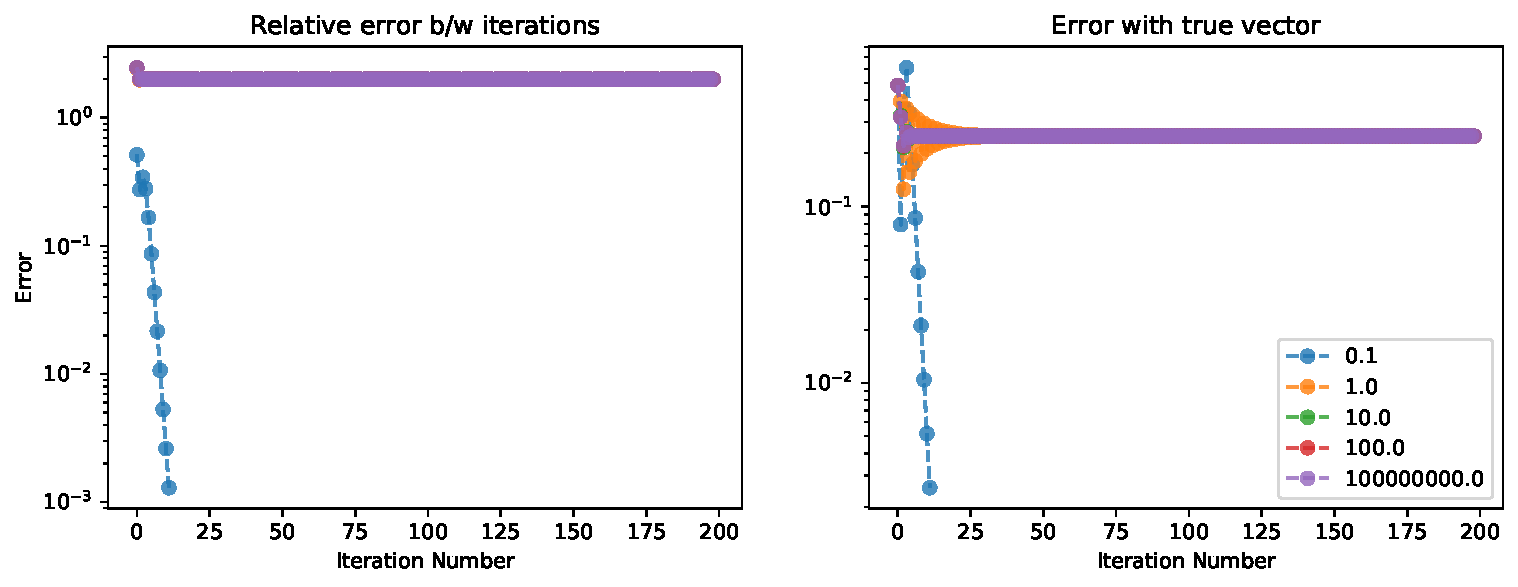
\includegraphics[width=200pt]{figures/random_init_2.pdf}
	\caption{First matrix: relative and absolute errors  $\| x_k - x_{k+1}\|_2$} on the left,  $\| |x_k| - |u_1| \|_2$ on the right
	\label{fig1}
\end{figure}

\begin{figure}[H]
	\centering
	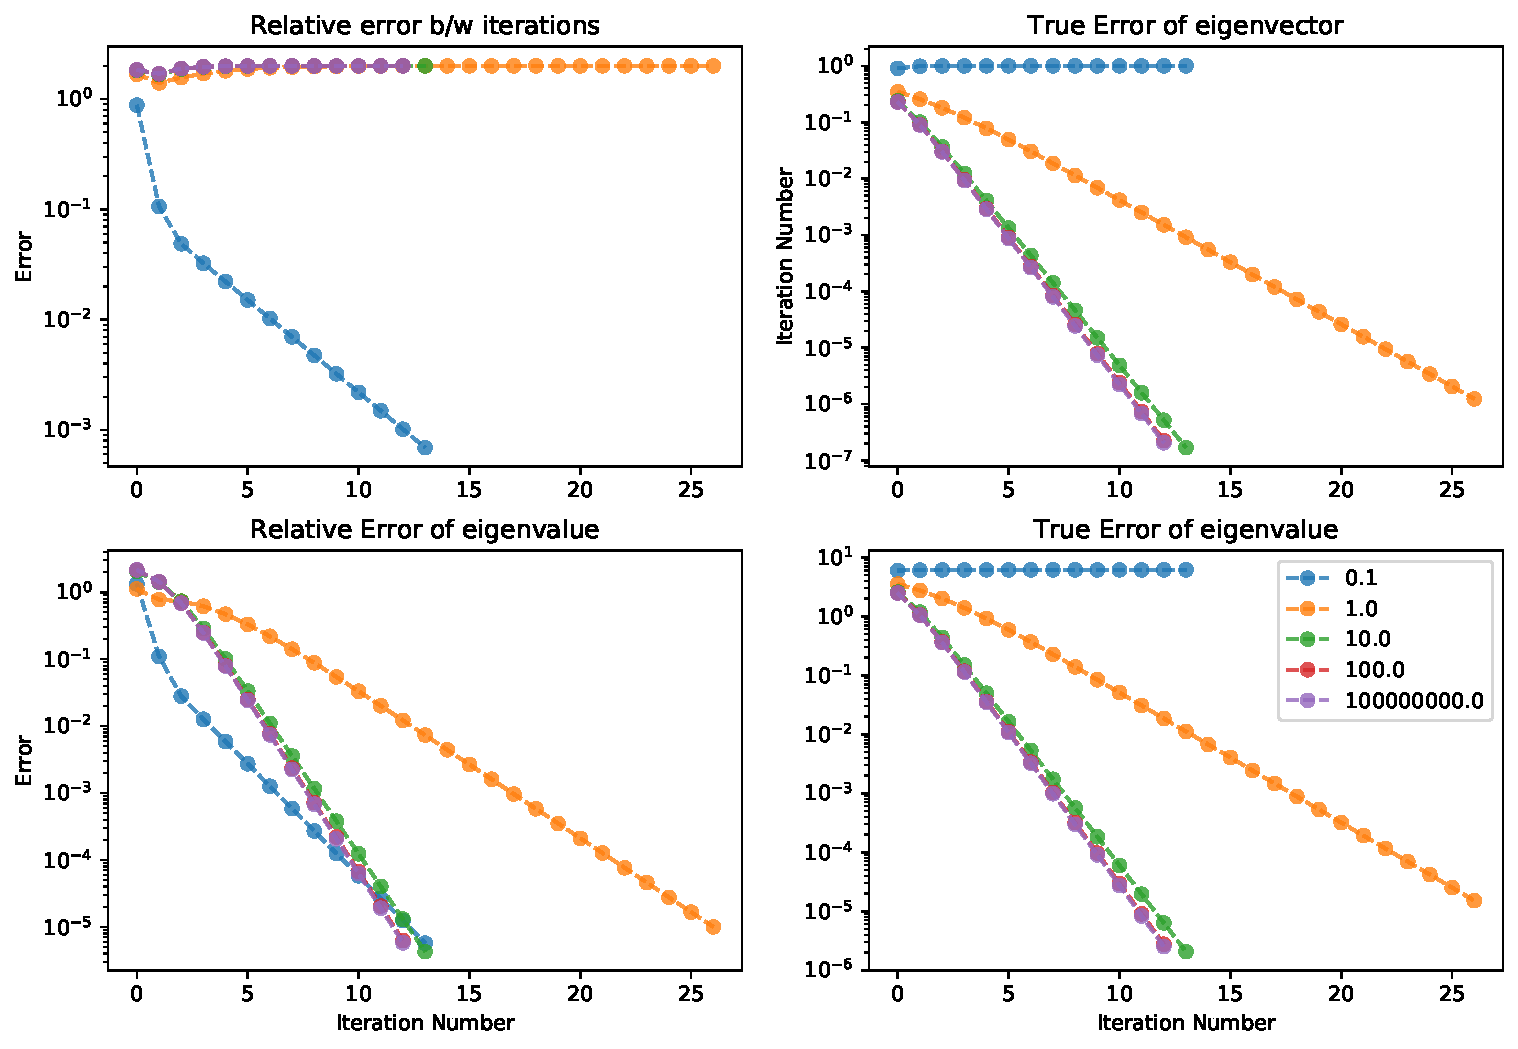
\includegraphics[width=200pt]{figures/random_init_3.pdf}
	\caption{Second matrix: relative and absolute errors  $\| x_k - x_{k+1}\|_2$} on the left,  $\| |x_k| - |u_1| \|_2$ on the right
	\label{fig1}
\end{figure}

\begin{figure}[H]
	\centering
	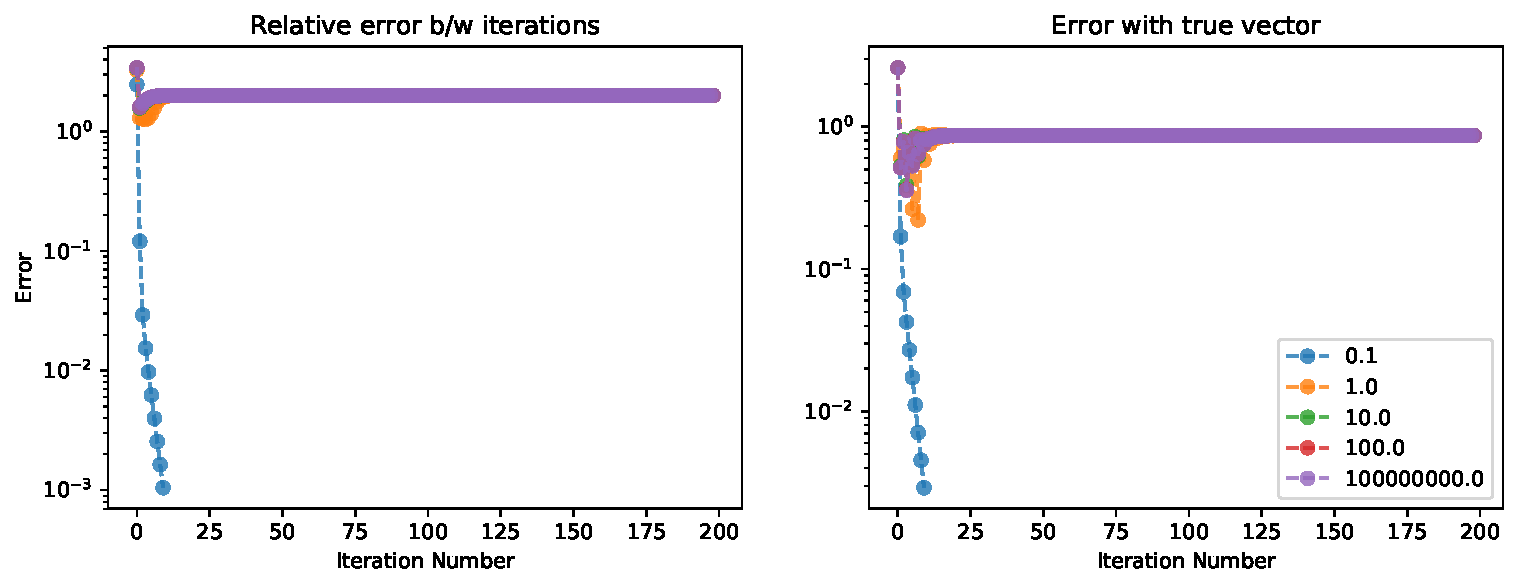
\includegraphics[width=200pt]{figures/random_init_4.pdf}
	\caption{Third matrix: relative and absolute errors  $\| x_k - x_{k+1}\|_2$} on the left,  $\| |x_k| - |u_1| \|_2$ on the right
	\label{fig1}
\end{figure}

We also observe that the initial point plays a role on how fast there is convergence to a stable state from one iteration to the other:

\begin{figure}[H]
	\centering
	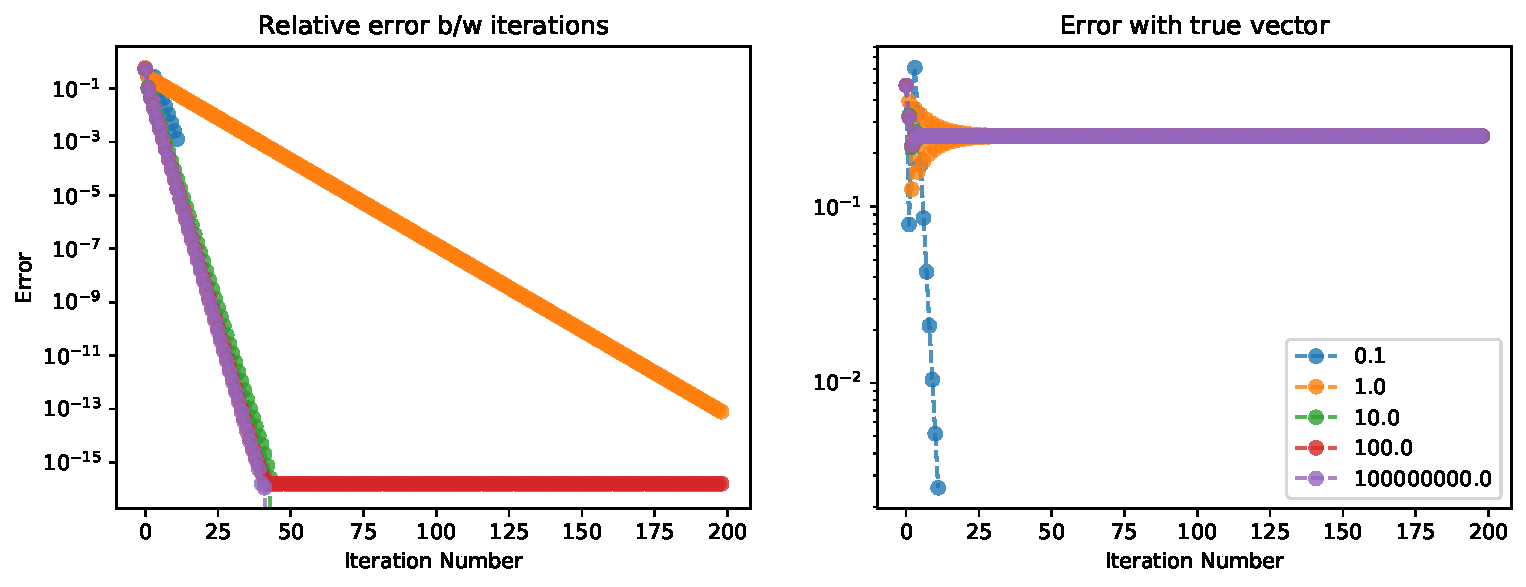
\includegraphics[width=200pt]{figures/random_init_2_abs_error.pdf}
	\caption{First matrix: relative and absolute errors  $\| |x_k| - |x_{k+1}| \|_2$} on the left,  $\| |x_k| - |u_1| \|_2$ on the right
	\label{fig1}
\end{figure}

\begin{figure}[H]
	\centering
	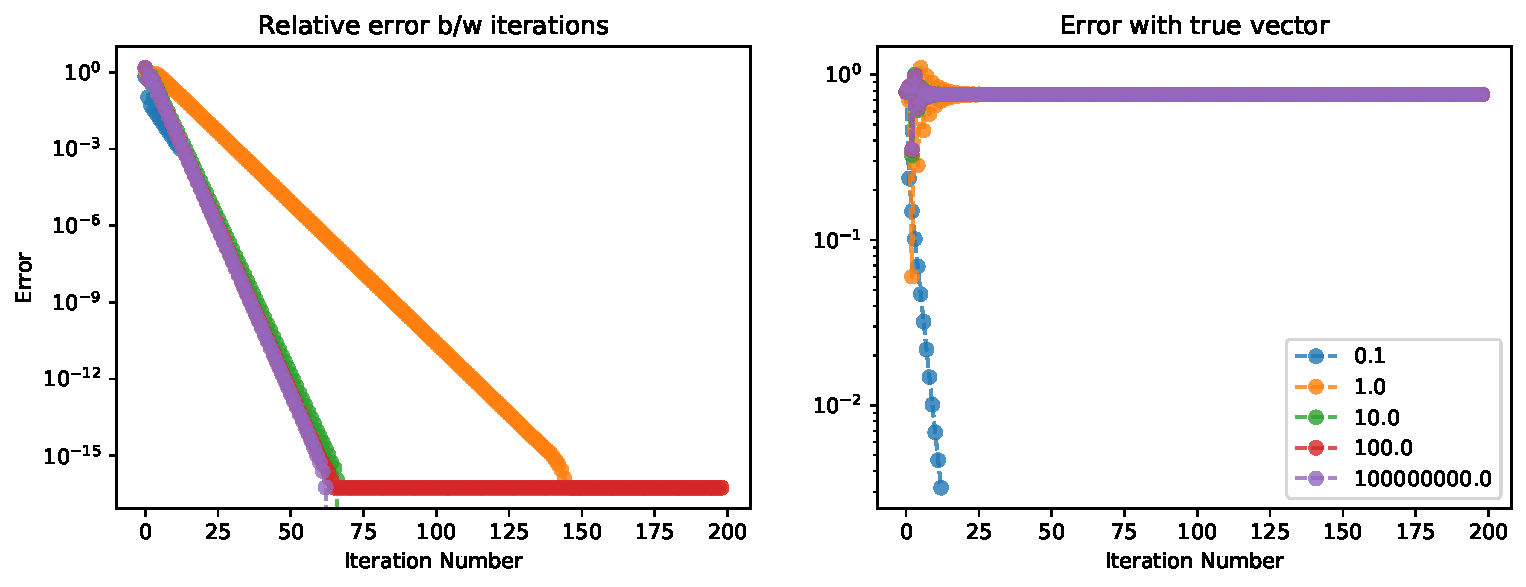
\includegraphics[width=200pt]{figures/random_init_3_abs_error.pdf}
	\caption{Second matrix: relative and absolute errors  $\| |x_k| - |x_{k+1}| \|_2$} on the left,  $\| |x_k| - |u_1| \|_2$ on the right
	\label{fig1}
\end{figure}

\begin{figure}[H]
	\centering
	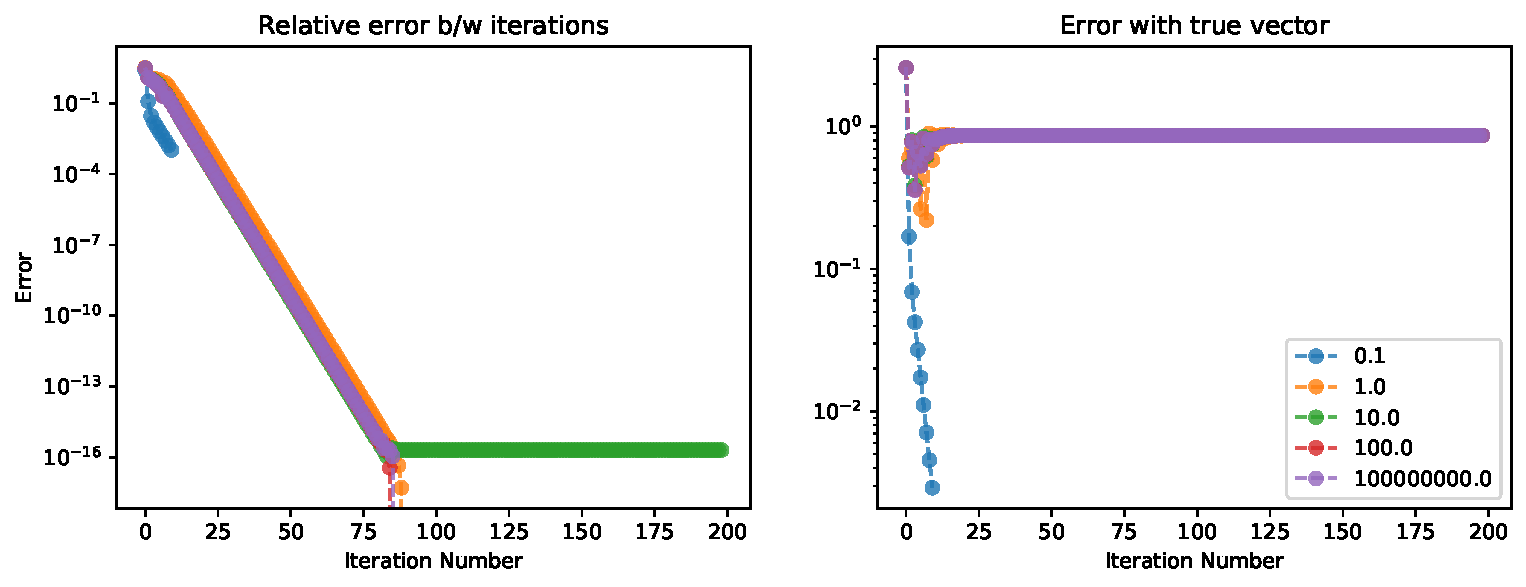
\includegraphics[width=200pt]{figures/random_init_4_abs_error.pdf}
	\caption{Third matrix: relative and absolute errors  $\| |x_k| - |x_{k+1}| \|_2$} on the left,  $\| |x_k| - |u_1| \|_2$ on the right
	\label{fig1}
\end{figure}

\end{enumerate}

\end{enumerate}

\end{document}
